\chapter{Assembling \& Debugging}

\section{nasm Assembly File Structure}

The entire assembly file structure introduced here is based on the \verb+nasm+ file
structure. 


In this section, we'll go through the basic structure of an Assembly file, and
in the following two sections, we will cover assembling it and debugging it. We
will be working on a template {\bf Hello World! } Assembly code as a sample, to
first learn the general structure of an assembly file and then how to assemble
it and debug it. Let us start by taking a look at and dissecting a sample Hello
World! Assembly code template:
\begin{verbatim}
         global  _start

         section .data
message: db      "Hello!"

         section .text
_start:
         mov     rax, 1
         mov     rdi, 1
         mov     rsi, message
         mov     rdx, 18
         syscall

         mov     rax, 60
         mov     rdi, 0
         syscall
\end{verbatim}

This Assembly code (once assembled and linked) should print the string 'Hello!'
to the screen. We won't go into detail on how this is processed just yet, but
we need to understand the main elements of the code template.

\subsection{Assembly File Structure}

 \begin{figure}
  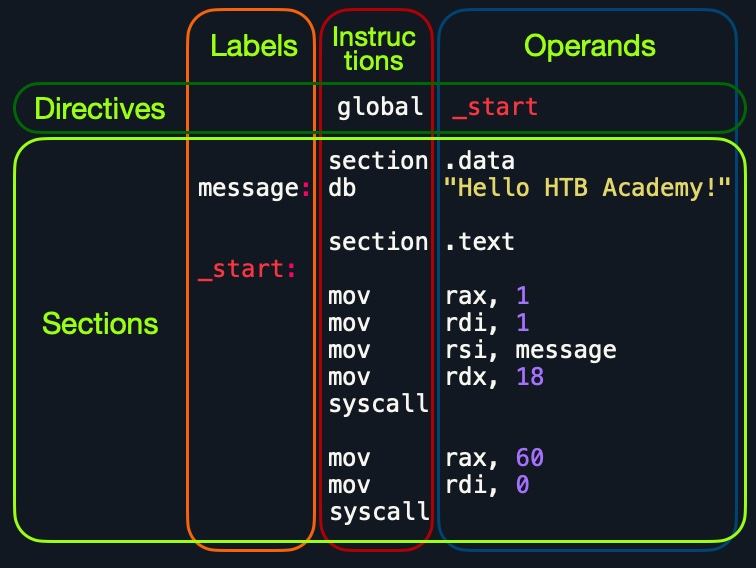
\includegraphics[width=\linewidth]{binary/assembly/images/nasm_structure.jpg}
  \caption{nasm structure}
  \label{fig:nasm_structure}
\end{figure}

Each label can be referred to by instructions or by directives.

The code is composed of three main parts:
\begin{verbatim}
Section 	    Description
global _start 	This is a directive that directs the code to start executing 
                at the _start label defined below.
section .data 	This is the data section, which should contain all of the variables.
section .text 	This is the text section containing all of the code to be executed.
\end{verbatim}

Both the \verb+.data+ and \verb+.text+ sections refer to the data and text
memory segments, in which these instructions will be stored.

\subsection{Directives}

An Assembly code is line-based, which means that the file is processed
line-by-line, executing the instruction of each line. We see at the first line
a directive \verb+global _start+, which instructs the machine to start
processing the instructions after the \verb+_start+ label. So, the machine goes
to the \verb+_start+ label and starts executing the instructions there, which
will print the message on the screen. This will be covered more thoroughly in
the Control Instructions sections.

\subsection{Variables}

Next, we have the \verb+.data+ section. The data section holds our variables to
make it easier for to define variables and reuse them without writing them
multiple times. Once we run the program, all of variables will be loaded into
memory in the data segment.

We can define variables using \verb+db+ for a list of bytes, \verb+dw+ for a
list of words, and so on. Variable  can be labeled  in order to be referenced.
The following are some examples of defining variables:
\begin{verbatim}
db 0x0a 	Defines the byte 0x0a, which is a new line.
message db 0x41, 0x42, 0x43, 0x0a 	Defines the label message => abc\n.
message db "Hello World!", 0x0a 	Defines the label message => Hello World!\n.
\end{verbatim}

Furthermore, we can use the \verb+equ+ instruction with the \verb+$+ token to evaluate an expression, like the length of a defined variable's string. 
\begin{verbatim}
section .data
    message db "Hello World!", 0x0a
    length  equ $-message
\end{verbatim}

\subsection{Code}

The second (and most important) section is the \verb+.text+ section. This
section holds all of the assembly instructions and loads them to the text
memory segment. Once all instructions are loaded into the text segment, the
processor starts executing them one after another.

The default convention is to have the \verb+_start+ label at the beginning of
the \verb+.text+ section, which -as per the \verb+global _start+ directive-
starts the main code that will be executed as the program runs. As we will see
later in the module, we can define other labels within the .text section, for
loops and other functions.

The text segment within the memory is read-only. 

The data section, on the other hand, is read/write but not executable, so any
code we write to it cannot be executed. This separation is part of memory
protections to mitigate things like buffer overflows and other types of binary
exploitation.

With this, we should understand the basic structure of an Assembly file.

\section{ssembling \& Disassembling}

\subsection{linux}
\begin{verbatim}
nasm -f elf64 helloWorld.s
ld -o helloWorld helloWorld.o
\end{verbatim}

\begin{verbatim}
objdump -M intel -d helloWorld
\end{verbatim}


\subsection{windows}
\url{https://sonictk.github.io/asm_tutorial/}

\section{x86 (32bits) instructions set architecture}
\url{https://www.intel.com/content/dam/www/public/us/en/documents/manuals/64-ia-32-architectures-software-developer-instruction-set-reference-manual-325383.pdf}{x86\_64 manual}

Intel instructions vary in size from one to fourteen bytes. The opcode (short
for operation code) is mandatory for them all and can be combined with other
optional or mandatory bytes to create advanced instructions.

\href{http://ref.x86asm.net/coder32.html}{list of all opcodes}


Most instructions have two operators (like \verb+add eax, ebx+), but some have
one (\verb+not eax+) or even three (\verb+imul eax, edx, 64+). Instructions
that contain something with \verb+dword ptr [eax]+ reference the double word
value at memory offset \verb+[XXX]+. Note that the bytes are saved in reverse
order in the memory as Intel uses Little Endian representation. 

\subsection{Address Pointers}

Wrapping brackets around an operand means that that operand is to be
dereferenced, as if it were a pointer in C. In other words, the brackets mean
that you are reading a value from (or storing a value into) that memory
location, rather than reading that value directly.

\begin{verbatim}
[] 
[rsp+10]
QWORD PTR [rsp]
[myvar]
\end{verbatim}



\subsection{Arithmetic operations}
\subsubsection{INC / DEC}

\begin{verbatim}
inc dest
dec dest
\end{verbatim}

\subsubsection{ADD / SUB}

\begin{verbatim}
add dest, src
sub dest, src
\end{verbatim}

Destination and source can be either a register,  a memory reference
(\verb+[esp]+)

The source can also be an immediate number.

\subsubsection{DIV / IDIV}

\verb+IDIV+ is the same as \verb+DIV+ but signed division.

\begin{verbatim}
div    divisor
idiv   divisor
\end{verbatim}

The dividend is always \verb+eax+ and that is also were the result of the
operation is stored. The rest value is stored in \verb+edx+.

\begin{verbatim}
mov eax, 65
mov ecx, 4
div ecx
\end{verbatim}

\subsubsection{MUL / IMUL}

\begin{verbatim}
mul value                ; *  eax by value
mul dest, value, value   
mul dest, value
\end{verbatim}

\subsection{Bitwise operations}

\begin{verbatim}
add dest, src
or dest, src
xor dest, src
not eax
\end{verbatim}

\subsection{Data moving}
\subsubsection{mov}
\begin{verbatim}
mov dest, src
movzx dest, src
movzx dest, src
\end{verbatim}

MOV moves data from source into destination. Both source and destination can be
register, or one of them register and the other one a memory reference. Both
cannot be a memory reference however.

The mov instructions come in many flavours, \verb+MOVS/MOVSB/MOVSW/MOVSD+ for
example copy a byte, word or dword from source to destination.

\begin{verbatim}
 +------------------+                  +------------+
 | Registers        |                  | Memory     |
 +------------------+                  +------------+
 | EAX = 0x00000000 |       0x00403A40 | 0x7C81776F |
 | EBX = 0x00403A40 |       0x00403A44 | 0x7C911000 |
 +------------------+       0x00403A48 | 0x0012C140 |
                            0x00403A4C | 0x7FFDB000 |
                                       +------------+
mov eax, [ebx+8]
# eax = 0x0012C140
\end{verbatim}

\subsubsection{lea}

Another instruction that can be used for data moving is the \verb+LEA+
instruction which  stands for “Load Effective Address” and the syntax looks like this:
\begin{verbatim}
lea eax, dword ptr[ecx+edx] ; This will store ecx+edx in eax
\end{verbatim}

\verb+lea+ loads a pointer to the specified value.


\begin{verbatim}
 +------------------+                  +------------+
 | Registers        |                  | Memory     |
 +------------------+                  +------------+
 | EAX = 0x00000000 |       0x00403A40 | 0x7C81776F |
 | EBX = 0x00403A40 |       0x00403A44 | 0x7C911000 |
 +------------------+       0x00403A48 | 0x0012C140 |
                            0x00403A4C | 0x7FFDB000 |
                                       +------------+
lea eax, [ebx+8]
# eax = 0x00403A48
\end{verbatim}

\subsubsection{xchg}

Swap data between two registers or addresses 	
\begin{verbatim}
xchg rax, rbx 
\end{verbatim}

\subsection{Branching}
Branching encapsulate all the instruction that will point the instruction
pointer (\verb+EIP+) to another portion of the code.

If we wanted to temporarily jump to a point and
then return to the original calling point, we would use functions.


\subsubsection{Unconditional}
\begin{verbatim}
jmp address
\end{verbatim}


\subsubsection{Conditional}
\begin{verbatim}
je  address
jle address
jz  address
...
\end{verbatim}

\begin{verbatim}
jz  	D = 0 	Destination equal to Zero
jnz 	D != 0 	Destination Not equal to Zero
js 	    D < 0 	Destination is Negative
jns 	D >= 0 	Destination is Not Negative (i.e. 0 or positive)
jg 	    D > S 	Destination Greater than Source
jge 	D >= S 	Destination Greater than or Equal Source
jl 	    D < S 	Destination Less than Source
jle 	D <= S 	Destination Less than or Equal Source
\end{verbatim}

Most instructions set one or more flags. Let’s revisit some of the instructions
we already looked at and see which flags they set:
\begin{itemize}
    \item \verb+ADD/SUB+ can set all of the Z, S, O, C flags (and some more
            that are of no interest to us right now) according to the result. 
    \item \verb+AND+ instruction however always clears the O and C flags, but
        sets Z and S flags according to the result.
\end{itemize}

Depending on which flags are set, a jump will either happen or not.

\subsubsection{cmp}

most of the time you will see an instruction \verb+CMP+ being used before a
jump. \verb+CMP+ is the ideal pre-branch instruction as it can set all the
status flags and is really fast. The syntax for \verb+CMP+ is: 
\begin{verbatim}
cmp dest, src
cmp rbx, 10
cmp rbx, rax
\end{verbatim}

This does not mean the other instructions cannot be used
before a jump, for example \verb+XOR+ occurs frequently but the most common is
the \verb+CMP+ instruction.



\subsection{Loop}
The \verb+loop+ instruction decrements \verb+ECX+ and jumps to the address
specified by \verb+arg+ unless decrementing \verb+ECX+ caused its value to
become zero. For example: 
\begin{verbatim}
mov ecx, 5
start_loop:
; the code here would be executed 5 times
loop start_loop
\end{verbatim}


\subsection{Stack management}

\begin{verbatim}
pop dest
push var/reg
\end{verbatim}

POP (PUSH) increments (decrements) the stack pointer (\verb+ESP+) to point to the new
top of the stack.

We will primarily be pushing data from registers into the stack before we call
a function or call a syscall, and then restore them after the function and the
syscall. This is because functions and syscalls usually use the registers for
their processing, and so if the values stored in the registers will get changed
after a function call or a syscall, we will lose them.

\subsection{Functions / syscall}

\subsubsection{Syscalls}
SYSCALL invokes an OS system-call handler at privilege level 0.


\subsubsection{call}
CALL is like a jump with several differences. A jump instruction loads an address into EIP and
continues execution from there. A CALL however stores the current EIP on the stack, with
the expectation to reload it once the calleé (that is the called function) is done. A jump
instruction has no way to do that as the current position of the EIP is not
stored.

\begin{verbatim}
 CALL _function
\end{verbatim}

\subsection{Interrupts, Debugger traps}

 \begin{verbatim}
 int num    ; were “num” represents an interrupt handler
 \end{verbatim}

Interrupts are used to tell the CPU to halt the execution of a thread. They can
be hardware based, software based or exception based (for example unauthorized
memory access attempt). When the INT instruction is hit, the execution is moved
to an exception handler, which is defined by num. Some INT flavours do not
require a num value, INT3 for example.

When a software based breakpoint is set in an assembly level debugger the
instruction where the breakpoint is supposed to hit is exchanged to an int3
instruction, which has the hexadecimal value of \verb+0xCC+. And when the
interrupt is hit, the control of the thread is handed back to the debugger. At
the same time, the {\bf trap flag} is set. When a program is single stepped in a
debugger, the CPU is checking for the trap flag. If the trap flag is set, the
CPU will execute one instruction and give control of the thread back to the
debugger.

Again, there are other flavours of breakpoints like conditional breakpoints,
memory breakpoints and hardware breakpoints. This was just a detailed
explanation of software breakpoints to demonstrate the idea of breakpoints.

\section{x64 instruction set architecture}

x64 is a generic name for the 64-bit extensions to Intel's and AMD's 32-bit x86
instruction set architecture (ISA)



